 \documentclass[5]{article}
\usepackage[utf8]{inputenc}
\usepackage{hyperref} 

\usepackage[T1]{fontenc}
\usepackage[polish]{babel}

\title{Laboratorium 6}
\author{Piotr Witek}
\date{28 kwietnia 2021}

\usepackage{natbib}
\usepackage{graphicx}
\usepackage{geometry}
\usepackage{tabularx}
\usepackage{array}
\usepackage{amsmath}

\begin{document}

\newgeometry{tmargin=2cm, bmargin=2cm, lmargin=2.5cm, rmargin=2.5cm}

\maketitle


\section{Zadania -gsl}

\hspace{4mm} Użyto następujących metod interpolacji podstawiając za gsl\_interp\_type: 
\begin{enumerate}
    \item gsl\_interp\_linear
    \item gsl\_interp\_polynomial
    \item gsl\_interp\_akima\_periodic
\end{enumerate}

\begin{center}
    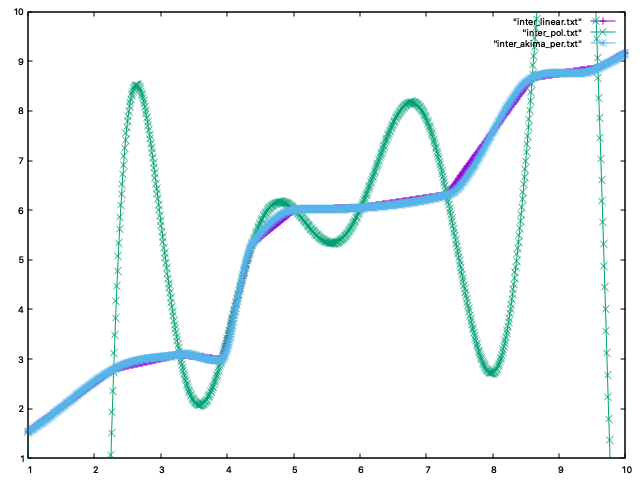
\includegraphics[scale=0.6]{zad1_2.png} \par
    \vspace{3mm}
    
\end{center}

\newpage

\section{Zadania - gnuplot}

\subsection{Dane zgromadzone w pliku dane1.dat}

\hspace{4mm} Oś x musi mieć skalę logarytmiczną:
\begin{verbatim}
gnuplot> set logscale x
gnuplot> plot "dane1.dat.txt"
\end{verbatim}

\begin{center}
    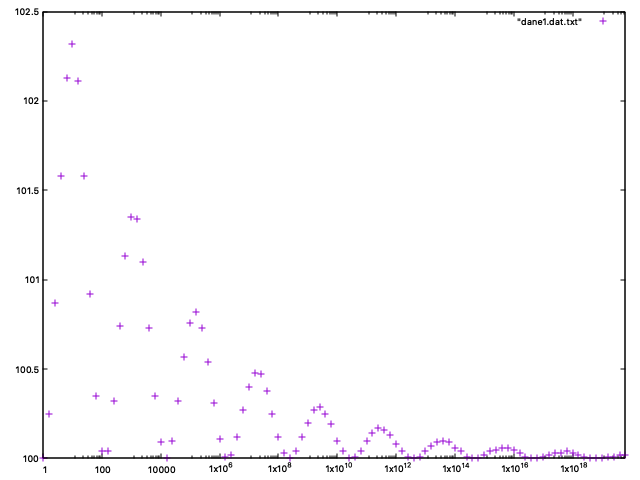
\includegraphics[scale=0.7]{zad2.png} \par
    \vspace{3mm}
\end{center}

\newpage
\subsection{Dane zgromadzone w pliku dane2.dat}

\hspace{4mm} Ustawienie strzałki na maksimum: 
\begin{verbatim}
set arrow 3 to 4,3,1
\end{verbatim}

Rysowanie wykresu:
\begin{verbatim}
set dgrid3d 30,30
set hidden3d
splot "dane2.dat.txt" u 1:2:3 with lines
\end{verbatim}

\begin{center}
    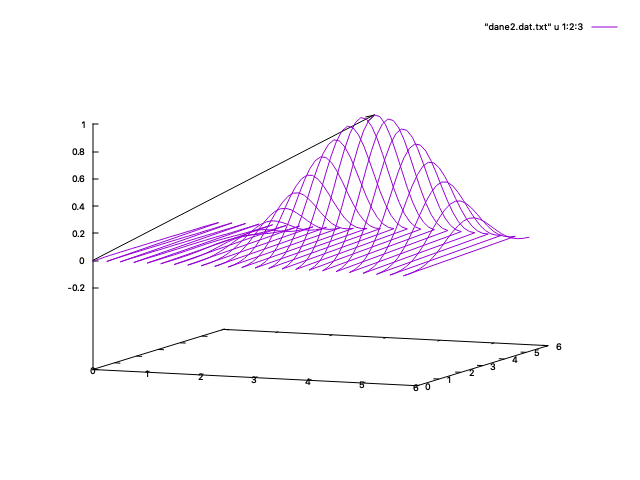
\includegraphics[scale=0.6]{zad3_with_arrow.png} \par
    \vspace{3mm}
\end{center}

\subsection{Odtworzenie wykresu z rysunku: }

\hspace{4mm} Ustawienie lokalizacji legendy oraz podpisu osi i wykresu: 
\begin{verbatim}
set key box left top width 2 height 2 opaque
set title 'Wykres testowy'
set ylabel 'Amplituda'
\end{verbatim}

Narysowanie wszytskich funkcji: 
\begin{verbatim}
plot [-3:3][-4:5]
"fun1.txt" using 1:($2+$3)/2:2:3 title "Dane z pliku fun1.txt" w yerrorbars lt rgb "red" lw 2,
sin(x**5) title "funkcja 2: sinus(x^5)" with lines lt rgb "green" lw 2,
3*sin(x) title "funkcja 3: 3*sin(x)" lt rgb "red"lw 2,
2*cos(x*sin(x)) title "funkcja1: 2*cos(x*sin(x))" w boxes lt rgb "blue"
\end{verbatim}

\begin{center}
    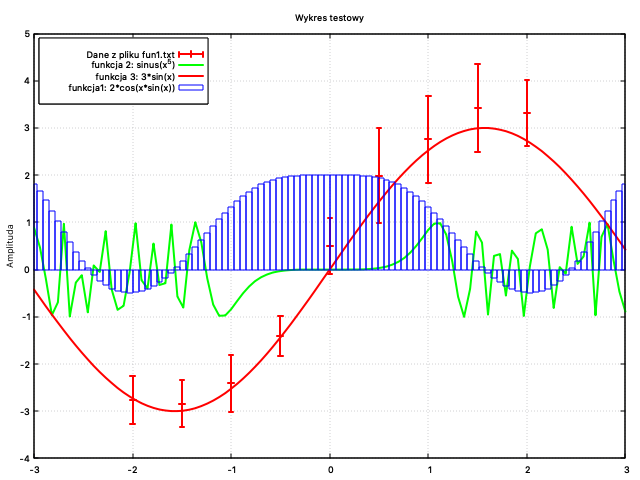
\includegraphics[scale=0.7]{zad4.png} \par
    \vspace{3mm}
    
\end{center}



\section{Bibliografia}

\begin{enumerate}
  \item \url{https://www.gnu.org/software/gsl/doc/html/interp.html}
  \item \url{http://people.duke.edu/~hpgavin/gnuplot.html}
  \item \url{https://www.gnu.org/software/gsl/doc/html/}
\end{enumerate}

\end{document}
